\documentclass[a4paper,12pt]{article} 
\usepackage[francais]{babel}
\usepackage[T1]{fontenc} 
\usepackage[utf8]{inputenc} 
\usepackage{graphicx}
\usepackage{color}
\usepackage{hyperref}
\begin {document}
\begin {figure}
\includegraphics[width=0.3\textwidth]{logolemansU.png}
\hspace{150pt} 
\includegraphics[width=0.3\textwidth] {logo_ic2.png}
\end {figure}
\title {\textbf {\color {blue} Le Mans Université}\color{black}
\\  Licence Informatique  \textit {2ème année}
 \\Module projet
 \\ \textbf {Bataille navale : https://github.com/KillianDEUX/bataille-navale}}
\author{DEUX Killian & GERARD Jules & DEROUET Corentin}
% \author{\href{mailto: prenom.nom.etu@univ-lemans.fr} {prenom.nom.etu@univ-lemans.fr}}

\date{\today} 
\maketitle 
\newpage
\tableofcontents
\newpage


 
\section {Introduction}
 	Dans le cadre de l'unité d'enseignement \og Conduite de projets \fg{}, nous avons du programmer un jeu en langage C à plusieurs. \vspace{2\baselineskip}\\
    L'objectif de ce projet est de mettre à contribution les enseignements appris depuis le début de notre cursus comme \og Algorithmique \fg{}. Cela a permis de nous former au travail en groupe, une nouveauté pour nous.
    \vspace{2\baselineskip}\\
    Nous avons choisi comme sujet la \og bataille navale \fg{}. C'est un jeu de société qui, dans sa forme originale, se joue à deux joueurs dans lequel chacun d'entre eux doivent placer des bateaux sur une grille, inconnue de l'adversaire. La partie se termine quand l'un des joueurs trouve l'ensemble des bateaux de son adversaire avant que tous les siens ne soient découverts. \vspace{2\baselineskip}
    
    Chaque joueur dispose alors de deux grilles. La première servira à placer les bateaux et la seconde à placer des pions. Cette seconde grille sera une vue de la grille adverse.
        \vspace{2\baselineskip}\\
        Lors d'un tir à des coordonnées précises dans la grille adverse, l'ennemi indiquera si le tir a atterri \og dans l'eau \fg{}, a \og touché \fg{} ou a \og coulé \fg{} un bateau. C'est en fonction de ces informations que l'on peut placer un pion, de différente couleur en fonction du tir. Afin d'enrichir le jeu, nous avons changé quelques règles  définies en début de projet. \\
 
\newpage
\section {Organisation}
La planification du projet a été articulée autour de l'outil "Projects" de GitHub.\\
Celui-ci permet, via un système de "cartes", d'assigner des tâches à chaque membre du groupe.\\
\begin{center}
  \includegraphics[width=1\textwidth] {capture_projects.png}  
  Figure 1 - Planificateur GitHub 
\end{center}
De plus, l'outil "Code" permet de récupérer et de mettre à jour les changements effectués dans les différents fichiers.\\
\\
La répartition globale est la suivante :\begin{itemize}
\item Killian : gestion des bateaux et des opérations sur les matrices 
\item Corentin : gestion des matrices de pions et du mode jeu IA
\item Jules : protocole de communication et gestion du réseau 
\end{itemize}

\newpage
\section {Conception/Analyse}
\subsection {Explication des règles}
    Les règles de la bataille navale dans l'introduction sont fixes. Or nous voulions pouvoir adapter celles-ci aux exigences du ou des utilisateur(s). \\ Ainsi celui-ci est en mesure changer les règles basiques pour chaque partie de jeu qu'il souhaite effectuer. Certaines règles restent inchangées : deux bateaux ne peuvent ni se toucher ni se croiser ni être placé en diagonale. \\ Le joueur ne peut pas tirer deux fois au même endroit car la case contient déjà un pion et donc ne peut pas bouger ses bateaux de place au cours de la partie.\vspace{2\baselineskip}\\ Les modifications sont :
            \begin{itemize}
                \item changement de la taille du plateau de joueur ,
                \item choix du nombre de bateaux en fonction de la taille du plateau choisi précédemment :
                \item le nombre de joueur, de 1 à 5,
                \item  choix de la taille de chaque bateau, mais toujours définie entre 1 et 5. 
            \end{itemize} 
            \vspace{2\baselineskip}
        Chaque bateau de taille différente possède un type particulier, respectivement: 
            \begin{itemize}
                 \item Mine,
                 \item Torpilleur,
                 \item Sous-Marin,
                 \item Croiseur,
                 \item Porte-avion. \\
            \end{itemize}
     

     \newpage
     Pour calculer le nombre de navires pour une grille variable, une fonction a été utilisée.\\
      Ci-dessous la courbe obtenue avec Geogebra en fonction de 3 points. Les X sont déterminés par la taille de la matrice et les Y par le nombre de bateaux maximum voulu. Les 3 points sont donc 2 bateaux pour une matrice de 5x5, 5 bateaux pour une matrice de 10x10 et finalement 20 bateaux pour une matrice de 20x20. \\
      \begin{center}
         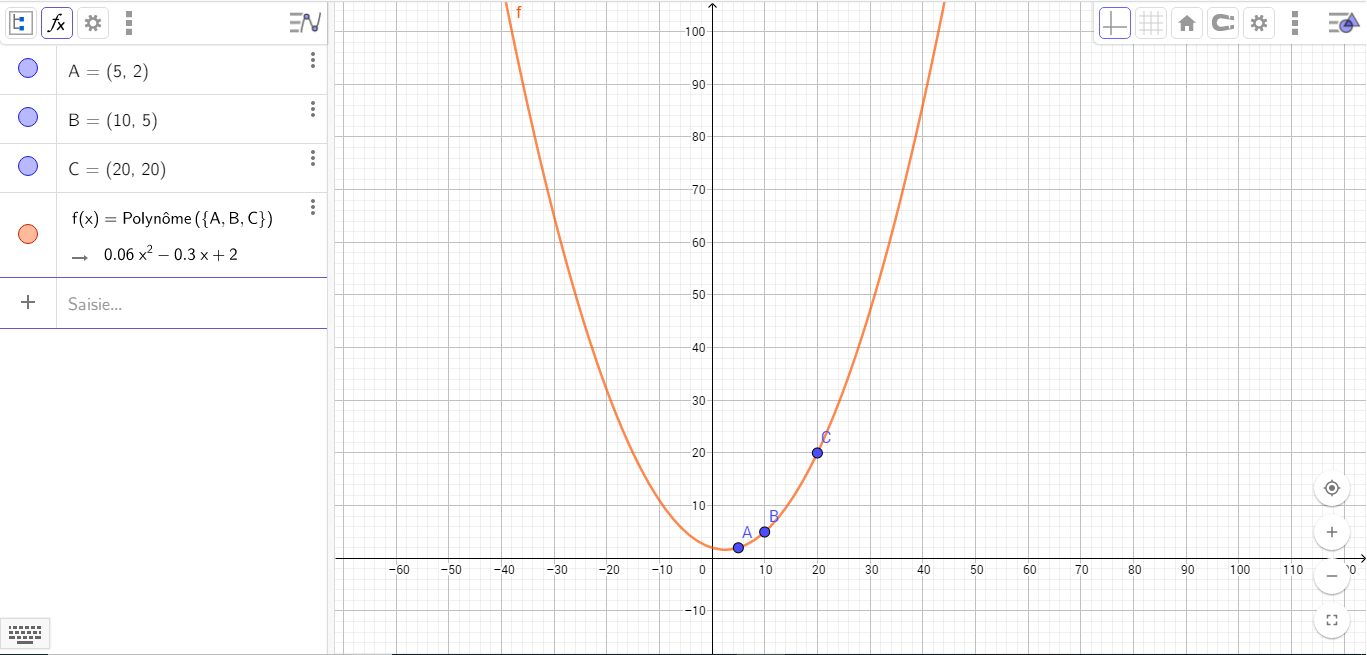
\includegraphics[width=1\textwidth] {courbe.png}
         Figure 2 - Courbe Geogebra
      \end{center}
      \newpage
\subsection {Explication des fonctionnalités}
        En fonction des nouvelles règles ajoutées et des règles basiques de la bataille navale, nous avons dû adapter notre code.
    \vspace{2\baselineskip}\\
    Le choix des cases se fait par lettre et chiffre. Pour une question de practicité, les cases sont numérotées, en ligne et en colonne, de 1 à n et de 1 à m (n et m étant demandés au joueur).\\
                Le joueur peut également choisir un plateau de jeu carré ou non. 
                \vspace{2\baselineskip}\\
                Comme l'énoncent les règles de l'introduction, chaque joueur possède 2 plateaux. L'un comprenant ses bateaux et l'autre, ses cases attaquées. 
                    Chaque case du plateau bateaux possède une cacactéristique, soit :
                    
                    \begin{itemize}
                        \item une case est vide,
                        \item une case touchée,
                        \item un bateau normal,
                        \item un bateau touché,
                        \item un bateau coulé.
                    \end{itemize}
                    \vspace{2\baselineskip}\\
                    Et chaque case du plateau adversaire possède d'autres caractéristiques, soit:\begin{itemize}
                        \item pas de pion,
                        \item un pion blanc,
                        \item un pion rouge.
                    \end{itemize}
\newpage
\section {Développement}
\subsection {Présentation de la conception d'un bateau}
\subsubsection{Présentation d'un bateau}
    Un bateau est constitué de :  
    \begin{itemize}
     \item sa taille 
     \item son type 
     \item ses premières coordonnées (là où il débute) 
     \item sa direction (verticale ou horizontale)
     \item son état (touché ou coulé) 
     \item nombre de fois qu'il a été touché par un joueur adverse
     \end{itemize}
    \\Toutes ses données sont nécessaires pour les traitements et utilisées tout au long du code.
\subsubsection{Présentation des listes de bateaux}
    Le premier joueur définit une série de bateaux qui sera reprise par les autres participants. Nous avons donc besoin de stocker ces bateaux dans des listes (vues au premier semestre) pour traiter efficacement ces éléments. Une liste possède un élément courant permettant de la parcourir ainsi qu'un "drapeau" signifiant la fin de celle-ci. Evidemment, nous avons dû adapter le système de listes pour qu'il soit applicable à nos bateaux.\\
\subsubsection{Fonctions de modification}
    Toutes les fonctions de modification de listes ou de bateaux sont placées dans des fichiers séparés pour une réutilisation facile.\\
    
    Lors de la mise en place des bateaux d'un joueur, une vérification est nécessaire concernant leur placement. La fonction parcours\_matrice est utilisée lors de ce processus. Elle parcourt la liste de bateaux déjà placés et récupère toutes les cases où le joueur ne pourra pas poser le navire. Donc pour chaque bateau, la fonction vérifie s'il est placé à la verticale ou à l'horizontale et parcourt toutes les cases autour de lui dans le but de les rentrer dans un tableau de cases non disponibles. 
    \newpage
    Une deuxième fonction appelée verif\_placement\_bateau, permet de vérifier que les coordonnées transmises, et donc souhaitées, n'interfèrent pas avec les coordonnées d'un autre bateau déjà placé. Donc pour chaque coordonnée voulue du bateau, la fonction parcourt entièrement le tableau de cases non disponibles. \\
    
\newpage
\subsection {Présentation des matrices}
    Nous avons eu besoin de créer deux types de matrices. La première matrice servira à placer nos propres bateaux, c'est la matrice "joueur". La seconde matrice servira à placer des pions en fonction de l'état du tir qui comprend trois choix possibles : touché, coulé ou dans l'eau. C'est la matrice "adverse". \\
    \subsubsection{La matrice "joueur"}
        La matrice "joueur" se compose d'un nombre de lignes et de colonnes renseigné par l'utilisateur en début de partie. Le joueur a le choix de donner une taille de grille minimale (5 lignes par 5 colonnes pour avoir un plateau jouable) et une taille maximale de 26x26. Les lignes étant modélisées par les lettres de l'alphabet. 
        
        
        Grâce à ces informations, le programme créé alors un tableau en conséquence. Chaque case sera initialisée avec des cases vides. Le premier joueur décide du nombre de bateaux et de leur taille pour tous les autres participants. Il place alors, en toute discrétion, ses propres bateaux en choisissant la direction et les coordonnées de chacun d'eux. Les autres joueurs ou l'intelligence artificielle placent ensuite leur flotte. Pour une meilleur compréhension par l'utilisateur, une légende est affichée. Celle-ci comprend la définition de chaque symbole en fonction de l'état de la case. Lors d'un tir d'un adversaire sur la flotte du joueur, les informations sur la case se mettent à jour. Les changements se font en même temps sur la grille adverse.\\
        \subsubsection{La matrice "adverse"}
            De plus, une autre matrice est créée. Il s'agit de la matrice adverse, elle possède la même taille que la matrice joueur. Cette matrice représente la vision partielle de la matrice de l'adversaire.
            
            Elle contient donc antant de lignes et de colonnes que la matrice "joueur". Pour bien différencier les deux types de matrices, l'affichage est complètement différent. Comme précedemment, la légende aide l'utilisateur à comprendre les tirs qu'il a fait sur la ou les grille(s) "adverse(s)". Une fois un tir effectué sur la grille de l'adversaire choisi (si un choix est possible), la case en question se transforme pour indiquer au joueur l'état de son tir. De plus avant chaque affichage de la matrice, le programe indique par une phrase si le tir est efficace ou nul. \\   
    
\subsection {Présentation des pions}
    La matrice "adverse" possède plusieurs caractéristiques. Les principales fonctionnalités de cette matrice sont d'indiquer l'état du tir et placer un pion, symbolisé par un caractère défini dans la légende en fonction de la case choisie. 
    \vspace{2\baselineskip}\\
    Une règle nous interdit de placer des bateaux les uns à côtés des autres. Pour faciliter l'expérience utilisateur, lorsqu'un bateau est touché, une fonction transforme toutes les cases autour comme 'dans l'eau'.
    \vspace{2\baselineskip}\\
    Une fois le bateau coulé, la fonction repère ce bateau, puis va sélectionner une par une chaque case présente autour et va remplacer le contenu de cette case par un pion "dans l'eau". Elle vérifiera cependant que la case est bien dans la grille car si un bateau est le long d'un bord, certaines cases autour se trouvent hors de la zone de jeu. \\ 
\newpage
\subsection {Présentation de l'Intelligence Artificielle}
    En temps normal, on ne peut pas jouer en solitaire à la bataille navale. Or une des fonctionnalités de notre code est le mode solo contre une IA. Cette IA se met en place lorsque le joueur indique qu'il veut jouer seul. 
\subsubsection {Placement des bateaux}
    L'IA place ses bateaux aléatoirement sur le plateau tout en vérifiant qu'aucun ne sorte de la grille ou ne touche un autre (en utilisant la même fonction que pour les joueurs).
\subsubsection {Choix des cases de tir}

    Lors de son premier tour, l'IA choisit une case du plateau aléatoirement. Puis, lors du tour suivant et pour tous les tirs, elle commence par vérifier si un bateau a déjà été touché et non coulé. \\
    Si c'est le cas, elle effectue un tir sur toutes les cases qui entourent le bateau déjà touché. Elle commence par les cases situées au nord de cette embarcation puis par l'est ensuite par le sud et pour finir, l'ouest. \\
    
    Si aucun bateau n'a été touché, l'IA choisit une case la plus éloignée possible de toutes les cases qui ont déjà été sélectionnées.\\
    Si aucune case n'a été trouvée, elle essaye de trouver une case pseudo aléatoirement. C'est-à-dire qu'elle trouve une case aléatoirement mais recommence tant qu'elle reste collée à une autre case déjà touchée.\\
    Si elle n'en trouve toujours pas, cette fois c'est une case totalement aléatoire qui est trouvée.
\newpage
\subsection {Présentation du réseau}
Dans ce mode de jeu, on dissocie deux exécutables : le serveur et les différents clients.
Le serveur, en plus de s'occuper des communications, présente une vue d'ensemble de la partie en cours. Le client propose l'interface de jeu.
\subsubsection {Serveur}
Pour permettre l'échange de données entre les différents utilisateurs, nous avons choisi d'implanter le réseau dans ce projet grâce au protocole TCP. Celui-ci présente un avantage important : le contrôle de l'information reçue.
    \vspace{2\baselineskip}
\\ Comme le jeu doit supporter un nombre variable de joueur, le serveur est en mesure d'ouvrir plusieurs sockets clients.
\\ Pour cela, il a été nécessaire de faire un tableau pour établir les canaux de communication de chaque client. Ainsi, le canal d’indice 0, correspond au 1er client qui s'est connecté et ainsi de suite.
      \begin{center}
         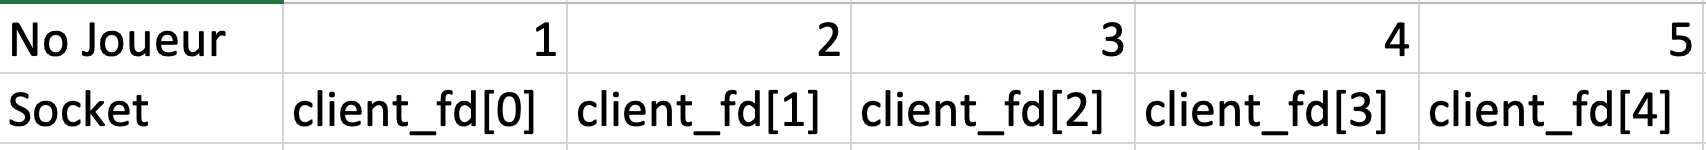
\includegraphics[width=1\textwidth] {tableau_clients.png}
         Figure 3 - Equivalence joueur et indice client
      \end{center}
       \vspace{2\baselineskip}
 Ces canaux vont permettre d'envoyer des variables par le réseau via les fonctions send et recv de la bibliothèque \og sys/socket.h \fg{}.
\\ Ce mode de fonctionnement est adapté au jeu de la bataille navale tour par tour car la fonction recv est bloquante. 
\\ La main est rendu à l’utilisateur dès que l'information est reçue, dans le cas contraire, celui-ci reste en attente.
    \vspace{2\baselineskip}
\\  Du coté client, un unique socket est établi vers le serveur. Les clients ne peuvent donc pas communiquer directement entre eux. Cette contrainte implique de nombreux envois.
\\ 
\newpage
\subsubsection {Clients}
Il est nécessaire de fournir l'information au client pour trouver le serveur. Notre choix s'est porté sur l'adresse IP pour plus de simplicité au lieu du nom d'hôte.
    Celle-ci est demandée à l'utilisateur avant d'initier la connexion. Le port est quant à lui défini en constante.
    \vspace{2\baselineskip}
\\  Pour plus de cohérence et d'équité, seul le premier joueur (le premier client connecté au serveur) choisi la taille de la grille et la liste de bateaux. Ces choix sont mémorisés et redistribués aux autres clients. Il leur reste la liberté de placer leurs navires.
    \vspace{2\baselineskip}
\\ Le mode de jeu réseau présente une spécificité : la grille de pions des joueurs ne varie pas en fonction du joueur attaquant mais en fonction du joueur attaqué.
\\ Ce choix, qui diffère de la règle originale, permet plus de stratégie lors des parties à plus de 2 joueurs.\\
\vspace{2\baselineskip}
\\ D'autre part, toujours dans le cas d'une manche à plus de 2 joueurs, le jeu s'achève lorsqu'un joueur a perdu l'intégralité de sa flotte.

\newpage
\subsection{Programmation modulaire}
\subsubsection{Fichiers utilisés}
    Pour pouvoir utiliser toutes nos fonctions de traitement comme par exemple le traitement des listes ou des bateaux, les fichiers générant l'IA ou encore les fichiers gestionnant les matrices de pions, un makefile est nécessaire.
    Le makefile demande la création de fichiers .h contenant la déclaration des structures, par exemple de quoi est composé un bateau, ainsi que les primitives de chaque fonction. \\
    Il permet de compiler, c'est-à-dire de transformer les fichiers, codés en language C, en fichiers contenant le language machine approprié. Ces fichiers transformés finissants par .o sont ensuite utilisés par le serveur et le client.
\subsubsection{Fichiers généraux}
    Le serveur et le client sont les deux fichiers utilisés par l'utilisateur lors de l'exécution. Pour jouer en solitaire et donc, contre l'IA l'exécution du serveur suffit. Sinon il faut exécuter le serveur ainsi que, pour chacun des joueurs, autant de client que de nombre de joueur. Chaque joueur ouvrant le sien. Le serveur et le client sont donc compilés en utilisant tous les fichiers .o nécessaires et générés précédemment. 

\newpage
\section {Résultat} 
A l'heure actuelle, le programme est fonctionnel et propose de manière indépendante les deux modes de jeu que nous souhaitions : solo contre l'IA et multijoueur en réseau. Les règles personnalisées sont toutes présentes, ce qui apporte un peu de nouveautés au jeu classique.
Néanmoins, certaines fonctionnalités n'ont pas été implémantées. 
\vspace{2\baselineskip}

    Le plus gros point noir est l'absence de l'interface graphique intialement prévue. Cette dernière aurait permis une bien meilleure expérience utilisateur. Par exemple, il aurait été plus naturel et ergonomique de devoir cliquer sur une case au lieu d'entrer des coordonnées au sein d'une console. 
        \vspace{2\baselineskip}

     Nous aurions également voulu ajouter un "timer" afin d'imposer une limite de temps sur un tour. Ainsi, l'attaquant qui dépasserait le temps imparti pour choisir sa cible serait obliger de passer son tour. Cette limite éviterait de trop longues attentes pour les autre(s) participant(s).
      
     \vspace{2\baselineskip}
    Une autre option qui avait été evisagée était de pouvoir déplacer un bateau au lieu d'attaquer un joueur. Cette option aurait rajoutée un aspect stratégique intéressant. Chaque joueur pourrait alors déplacer un bateau à condition qu'il ne soit pas déjà touché.
    
     
     \vspace{2\baselineskip}
      De plus, il serait intéressant que le mode de jeu IA puisse prendre la relève en cas d'un joueur réseau inactif ou encore en cas de perte de connexion.
      
    \vspace{2\baselineskip}
        Malgré quelques difficultés à la réalisation finale de notre code, nous avions l'idée, qui n'a malheureusement pas pu aboutir, de faire une bataille navale mais en 3D. C'est à dire avec plusieurs types de sous-marins ainsi que des avions. Donc le but était de faire 3 plateaux de jeu pour chaque joueur.
     
     
    \vspace{2\baselineskip}
    Enfin, il aurait été souhaitable, de mettre en place des pseudos et des highscores.

   
    
    


\newpage
\section {Conclusion} 
    Ce projet, assez conséquent, nous a permis de découvrir comment travailler à plusieurs. En effet, nous avons dû nous organiser et prévoir une répartition des tâches. 
    Les contraintes de temps ont été les plus difficiles. À cause de celles-ci, nous n'avons pas réussi à ajouter toutes les fonctionnalitées voulues, en particulier la SDL. Nous avons pourtant réussi à avoir un programme jouable sur terminal, que ce soit contre une IA ou en réseau, avec les règles prévues dans le cahier des charges. Même si, au niveau du réseau, l'optimisation n'est pas complète, il est quand même possible de jouer à la bataille navale jusqu'à 5 joueurs. Nous avons perçu les difficultés à travailler en groupe. \\

    Chaque personne travaillait sur une partie du code et lors de la mise en commun, même si nous nous étions mis d'accord sur des fonctionnalités, certaines fonctions n'était pas compatibles entre elles. A force de debogage, nous avons tout de même pu finir par avoir un jeu auquel il est possible de jouer. S'il fallait continuer ce projet, nous pourrions alors améliorer certains points importants comme l'interface et l'optimisation du réseau. Une fonctionnalité intéressante aurait été de ne pas arrêter la boucle de jeu lorsqu'un joueur perd. \\

\newpage
\section {Annexes}  
\begin{center}
    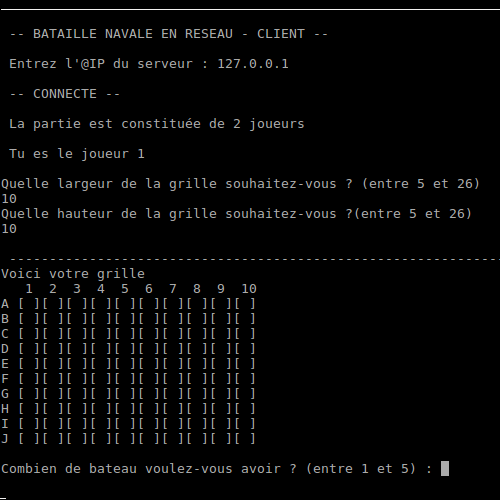
\includegraphics[width=1\textwidth] {capture_ecran_connexion_joueur1.png}  
    Capture d'écran de la connexion du joueur 1 au serveur \\
    \newpage
    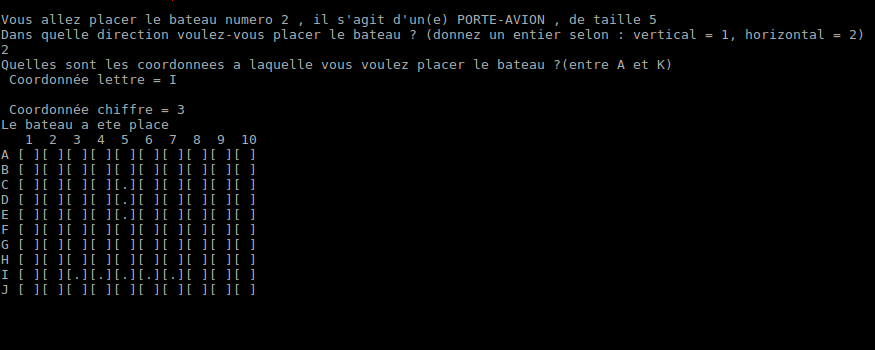
\includegraphics[width=1\textwidth] {Capture_ecran_placement_bateau.png}  
    Capture d'écran du placement de 3 bateaux
    \newpage
    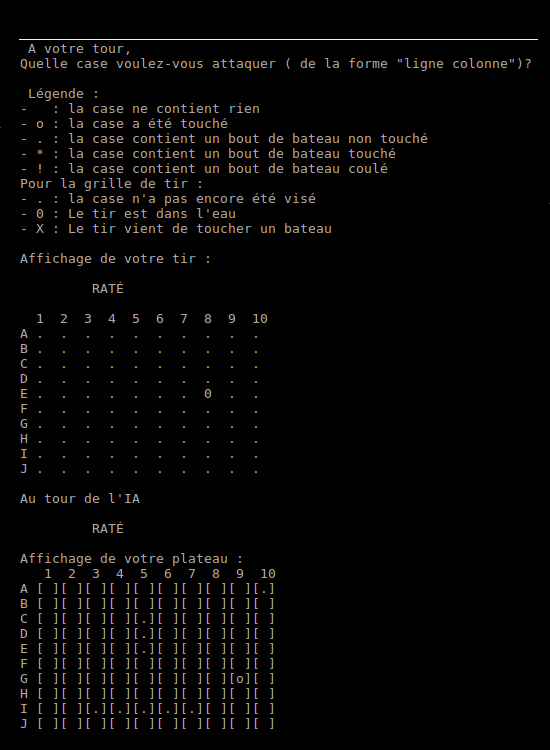
\includegraphics[width=1\textwidth] {capture_ecran_attaque_bateau.png}  
    Capture d'écran de l'attaque d'un bateau
    \newpage
    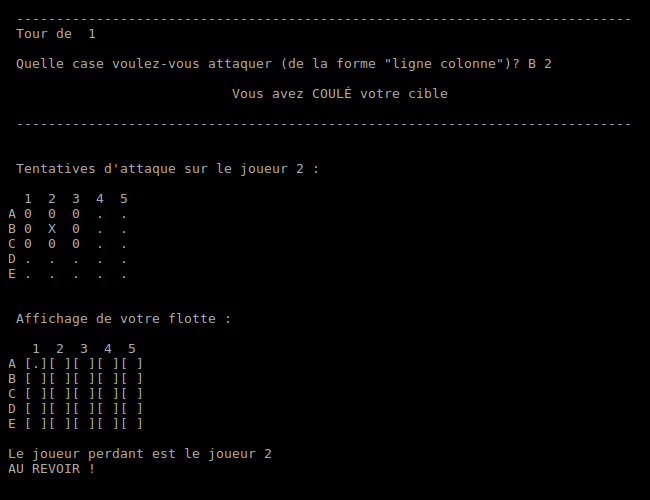
\includegraphics[width=1\textwidth] {capture_ecran_fin_de_jeu.png}  
    Capture d'écran de la fin de partie
\end{center}
\end {document}